\chapter{Materialien und Methoden}
\label{chap:methods}

\begin{mcimethods}
\section{Materialien und Geräte}
\offen{Gerätemodelle, Messbereiche, Auflösung, Kalibrierstatus und
Unsicherheiten dokumentieren. Für Chemikalien außerdem Bezeichnung,
Konzentration, Reinheit und eingesetzte Mengen ergänzen.}
Alle für die Reproduktion wesentlichen Angaben werden aus der tatsächlichen
Versuchsdokumentation übernommen.

\section{Versuchsaufbau}
In \figref{fig:setup} wird ein schematischer Beispielaufbau gezeigt.
Die Skizze wird vor der Abgabe durch den tatsächlichen, beschrifteten
Aufbau ersetzt.
\begin{figure}[htbp]
  \centering
  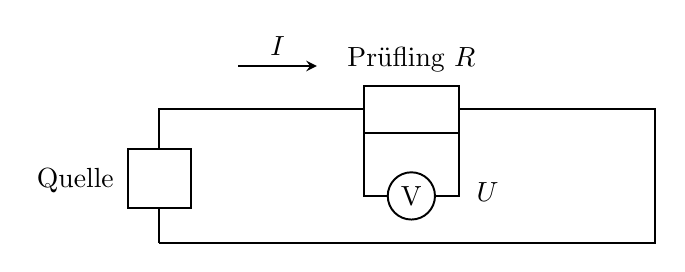
\begin{tikzpicture}[line width=0.7pt,>=stealth]
    \draw (0,0) -- (0,1.7) -- (2.6,1.7);
    \draw (3.8,1.7) -- (6.3,1.7) -- (6.3,0) -- (0,0);
    \draw[fill=white] (-0.4,0.45) rectangle (0.4,1.2);
    \node[left] at (-0.45,0.8) {Quelle};
    \draw[fill=white] (2.6,1.4) rectangle (3.8,2.0);
    \node[above] at (3.2,2.05) {Prüfling $R$};
    \draw[->] (1,2.25) -- (2,2.25) node[midway,above] {$I$};
    \draw (2.6,1.7) -- (2.6,0.6) -- (2.9,0.6);
    \draw (3.5,0.6) -- (3.8,0.6) -- (3.8,1.7);
    \draw[fill=white] (3.2,0.6) circle (0.3);
    \node at (3.2,0.6) {V};
    \node[right] at (3.9,0.65) {$U$};
  \end{tikzpicture}
  \caption[Beispiel einer Versuchsskizze]{Schematischer Beispielaufbau mit
    Quelle, Prüfling und Spannungsmessung. Eigene Darstellung; reale
    Gerätedetails und Strommessung ergänzen.}
  \label{fig:setup}
\end{figure}

\section{Durchführung und Auswertung}
\offen{Arbeitsschritte, Umgebungsbedingungen, Wiederholungen und
Auswertungsverfahren reproduzierbar beschreiben.}
Direkt erfasste Größen und berechnete Werte werden unterschieden.
Für jeden unterschiedlichen Rechenschritt wird ein Zahlenbeispiel gezeigt.
Ergänzende Unterlagen sind in Anhang~\ref{app:records} aufgeführt.
\end{mcimethods}
